\subsection{Structure and mechanics}

\textbf{INTRODUCCIÓ. FALTA!}

\begin{figure}[h]
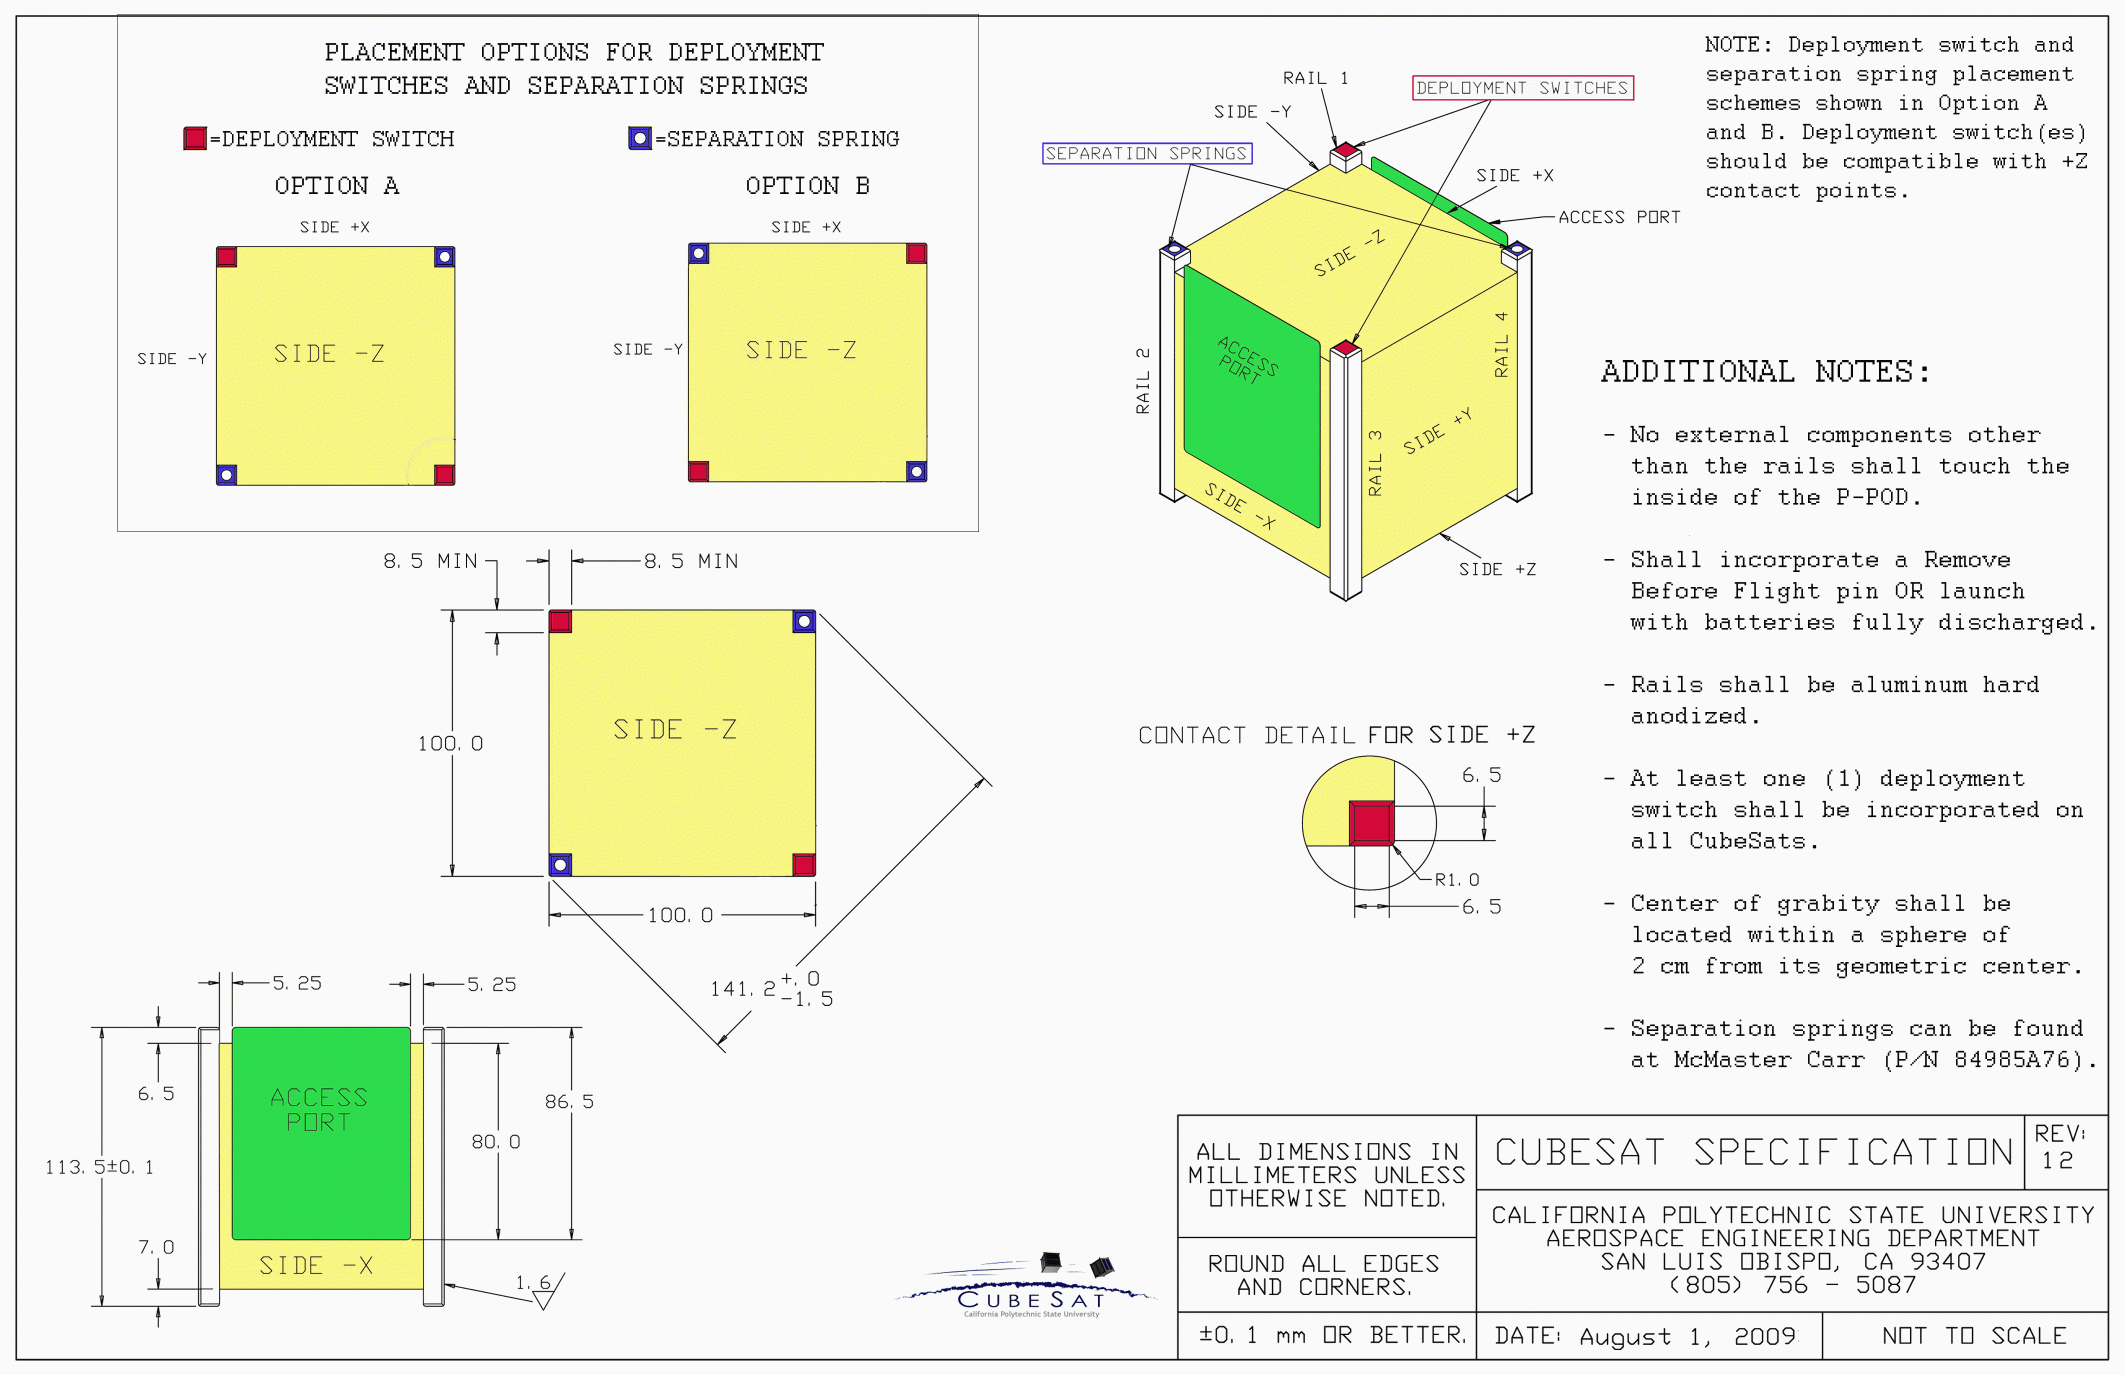
\includegraphics[scale=0.6]{./sections/SatelliteDesign/images/CubeSatDesign}
\centering
\caption{Dimensions of a 1U CubeSat \cite{cubesatdimensions}}
\end{figure}

\subsubsection{Structure}

\paragraph{}The mission of the structure is to sustain and protect all the electronic devices carried by the satellite in order to fulfill the mission requirements. In order to ensure that all the electronic and mechanic systems can be mounted upon the structure, a high compatibility between these systems is required.

The structure used will be provided by Innovative Solutions In Space (ISIS). Among its features it is worth mentioning that it can withstand the high range of temperature it will face in the space (-40ºC to 80ºC) and it is highly compatible with almost every physical system that will be used. Additionally, it is a low mass structure (304.3g) and it can support different configurations within it.

\paragraph{}Since the configuration within the CubeSat will not be as common as the other configuration within the current operational CubeSats, because the mission of our project is to relay fast and reliable communication with the ground station and the other satellites, it is a really important point that the structure is highly flexible regarding the arrangement of the subsystems that it will carry.

\subsubsection{Deployments}
EMPTY
\subsubsection{Thermal protection}
\paragraph{}The thermal protection system protect the CubeSat from thermal shocks. The satellite must remain in a optimal range of temperatures,despite the external temperature. It consists of various insulating materials and thermal conductors in order to maintain it within acceptable temperatures.

\subsubsection{Study of the commercial available options}
EMPTY

\begin{longtable}{| l | r | r | }
\hline
\rowcolor[gray]{0.80}	\textbf{System} &  \textbf{Brand and model}     & \textbf{Money (\euro)}   \\
\hline
\endfirsthead

	   ~3U Structure & ISIS & 3900) \\
	   ~EMPTY 1 & EMPTY & EMPTY \\
	   ~EMPTY 1 & EMPTY & EMPTY \\
	\hline

\caption{Options studied}
\label{epsoptionstable}
\end{longtable}

Of all the options in \ref{epsoptionstable}, we have chosen the following options.
